\chapter{Uživatelská příručka}

\section{Uživatelské role}

V systému Retrobi existují čtyři uživatelské role. Tyto role jsou uspořádány lineárně do hierarchie, přičemž vyšší role má vždy vyšší oprávnění než role nižší. 

Nejnižší rolí je {\em návštěvník} (GUEST). Tuto roli má každý člověk, který přijde na web, aniž by cokoliv musel dělat. Návštěvník má určitá omezení co se týče velikosti schránky a operací, které může provádět. To proto, aby každý náhodný návštěvník nemohl příliš zatížit systém a jeho paměť, protože těchto lidí bude pravděpodobně mnoho a mohli by zbytečně omezovat prostředky dostupné pro vážné zájemce či odborníky.

Další rolí je {\em uživatel} (USER). Uživatelem se lze stát po platné registraci do systému. Po přihlášení do systému Retrobi se uživatel vzdává své anonymity a jako náhradu získá vyšší limity pro velikost schránky a možnost provádět další operace. Zároveň si může ukládat např. své schránky do databáze. Uživatel může také začít přepisovat lístky, což mu bude započteno k dobru.

Ještě vyšší rolí je {\em editor} (EDITOR). Uživatele na editory povyšuje administrátor, například po schválení jeho kvalitních přepisů. Editor je tedy určitý privilegovaný uživatel, u kterého existuje jistá odbornost a zájem vylepšovat obsah databáze systému Retrobi. Editor může narozdíl od uživatele upravovat různé další parametry lístků a manipulovat s nimi v rámci katalogu. Také má přístup k některým částem správy - konkrétně k hromadné editaci a analýzám.

Nejvyšší rolí je {\em administrátor} (ADMIN). Administrátor může naprosto vše a jeho práci se neklade žádné omezení. Má například k dispozici celou sadu nástrojů na webovém rozhraní. Může také spouštět nástroje pro import dat. Při prvním spuštění systému je vytvořen výchozí administrátor s přihlašovacím jménem (loginem) {\tt admin} a heslem {\tt admin}. Tohoto prvotního administrátora můžete například použít pro spuštění nástrojů pro import dat (viz níže), další uživatelé se již mohou registrovat pomocí webového rozhraní.

\section{Skenování a import dat}

\subsection{Spuštění nástrojů}

Nástroje pro import naskenovaných dat se spouštějí z webu, a to ze sekce {\em Správa / Nástroje}. Tam jsou umístěny dva odkazy: {\em Stáhnout Udělátko 1} (přejmenování, konverze, detekce prázdných stran lístků) a {\em Stáhnout Udělátko 2} (zmenšení, zařazení, upload zpracovaných obrázků). Nástroje může spouštet jen uživatel s rolí {\em administrátor}. Výchozí administrátor je při prvním spuštění systému vytvořen s přihlašovacím jménem (loginem) {\tt admin} a heslem {\tt admin}.

Technicky je spuštění programů řešené přes dynamicky generované JNLP (technologie firmy Oracle, která umožňuje jednoduchým XML souborem definovat spuštění libovolné Java aplikace). Během generování tohoto souboru JNLP dochází i k injekci konfiguračních parametrů, jako je adresa databázového serveru, jméno a heslo. Technicky je sice možné spustit nástroje i pomocí příkazové řádky, ale právě z důvodu chybějící konfigurace se to nedoporučuje. Pokud však přesto chcete otestovat, jestli se vůbec nástroje alespoň spustí, můžete použít tyto příkazy:

\begin{verbatim}
(U1) java -cp retrobi-tools.jar 
 cz.insophy.retrobitool.processor.ProcessorMainFrame

(U2) java -cp retrobi-tools.jar 
 cz.insophy.retrobitool.importer.ImporterMainFrame
\end{verbatim}

\subsection{Stručný proces}

\begin{figure}
\label{fig:import}
\centering
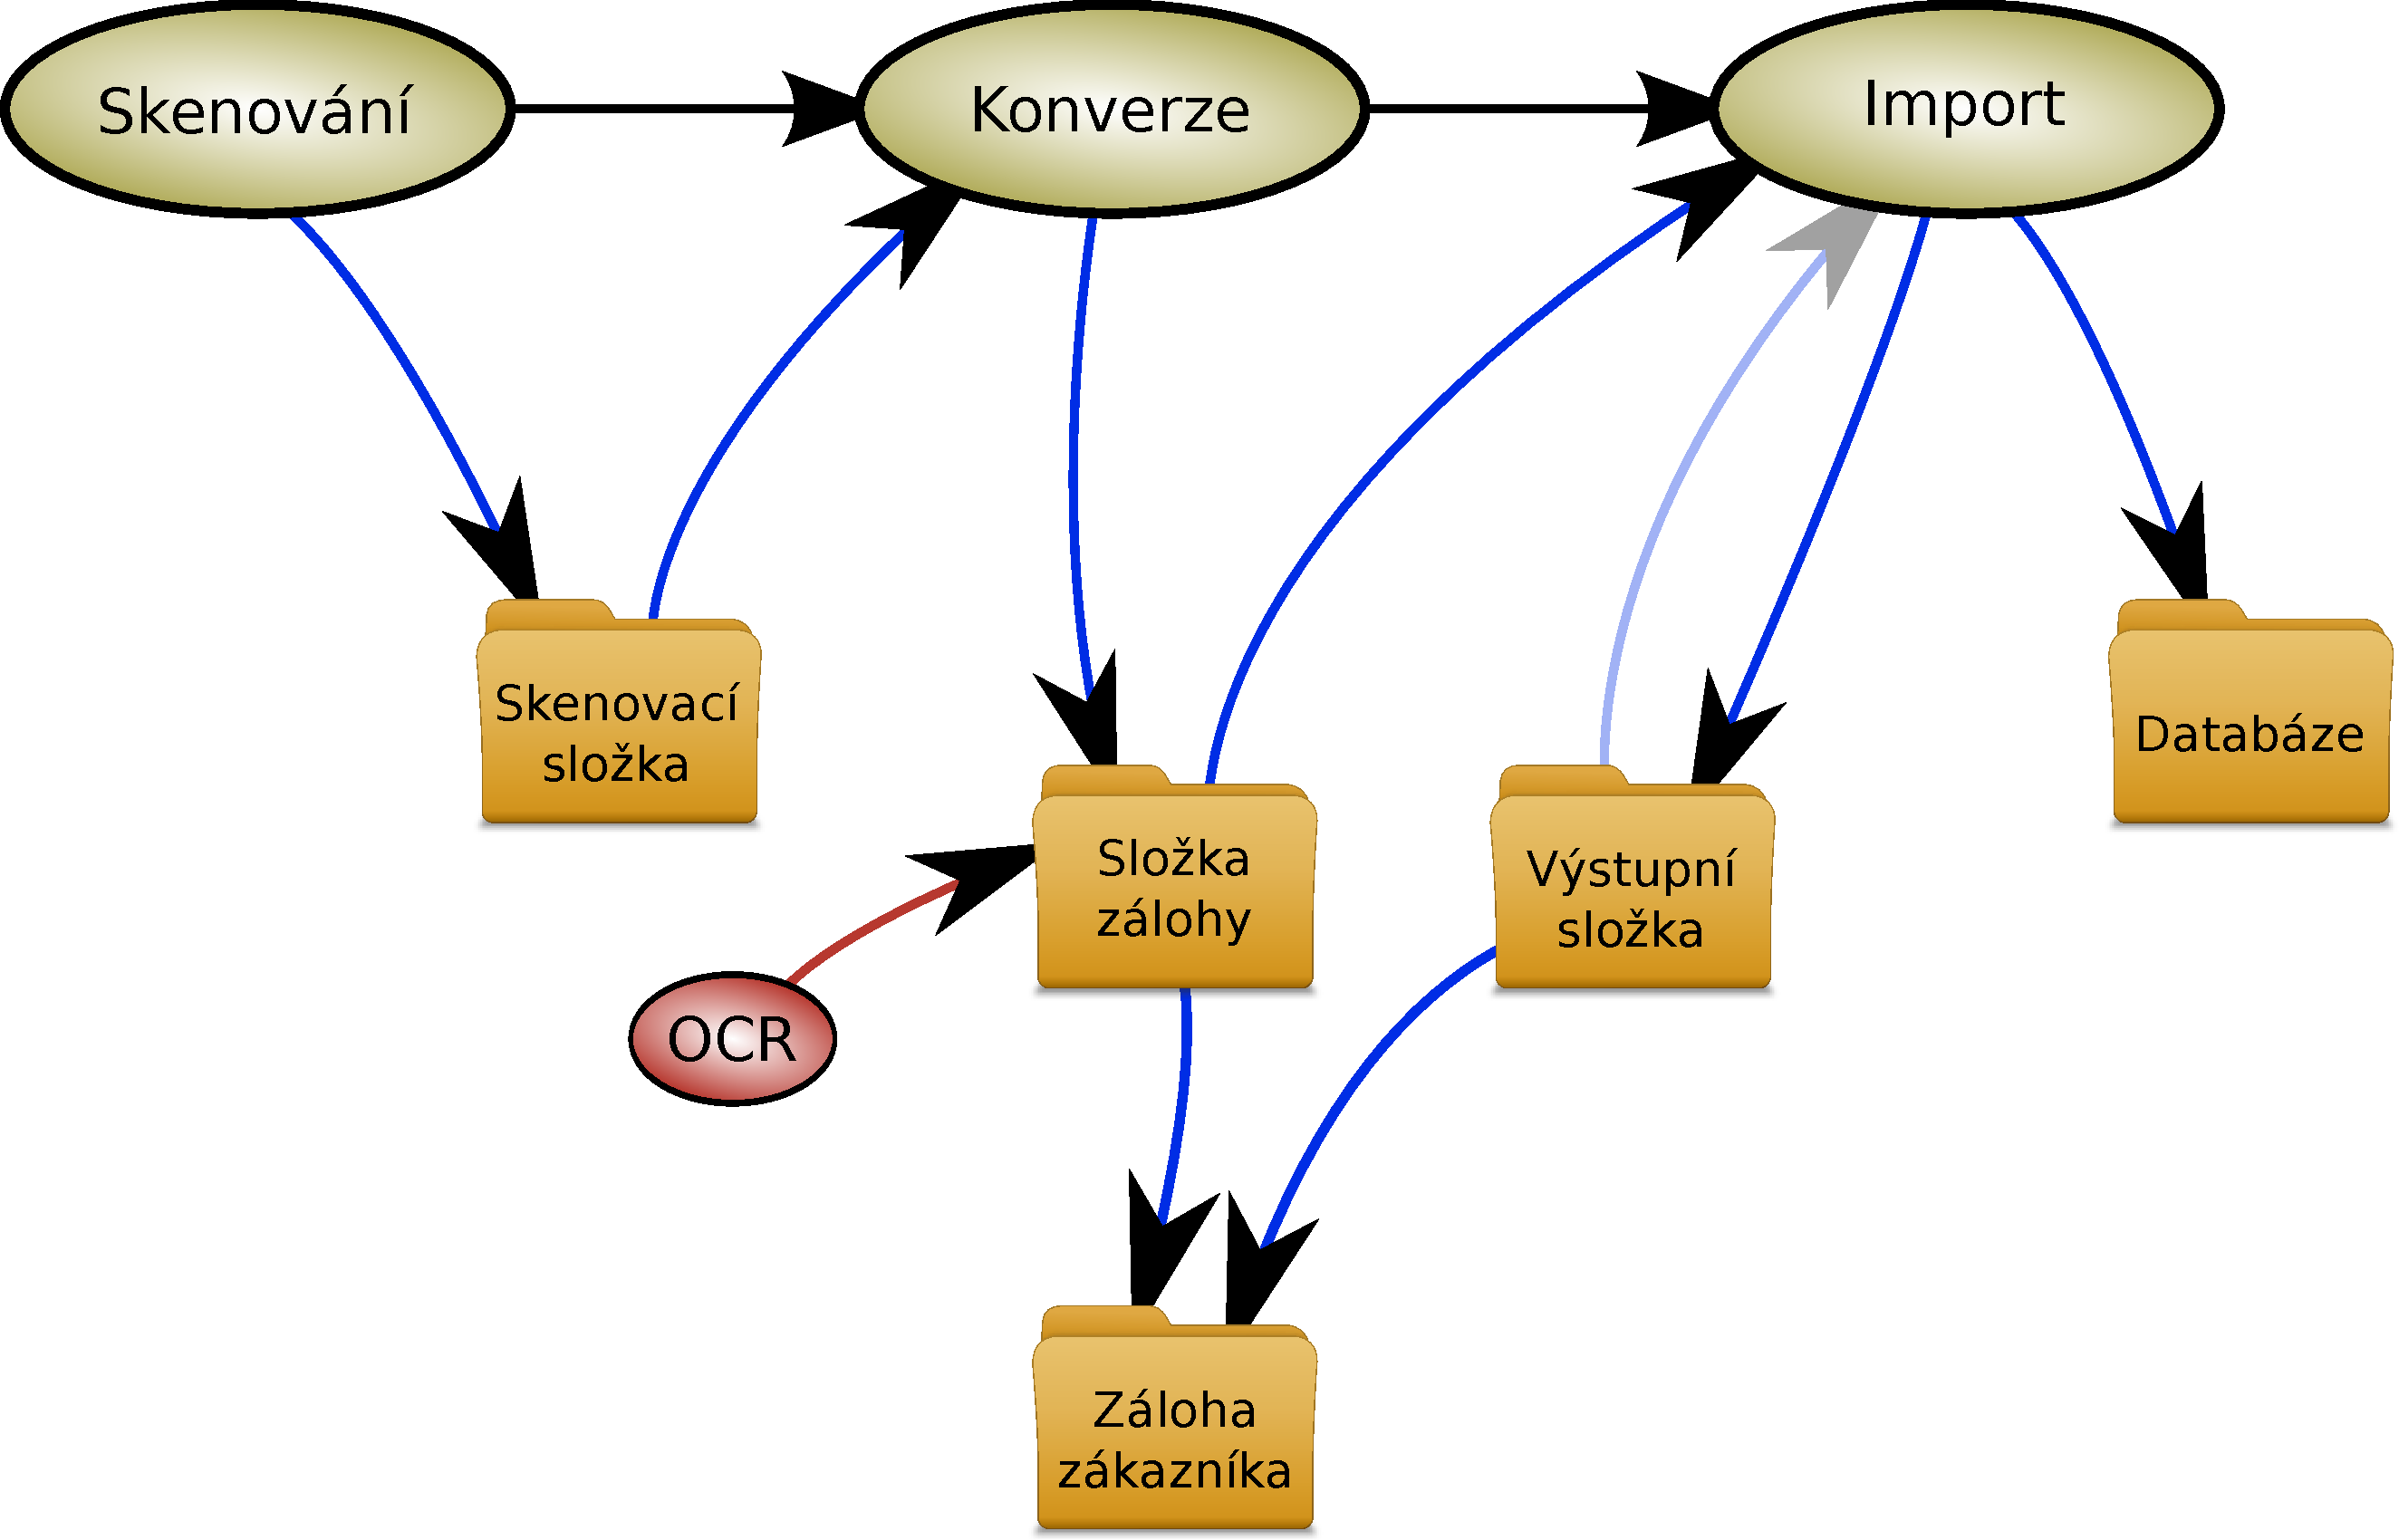
\includegraphics[width=.8\textwidth]{import.pdf}
\caption{Proces a tok dat během importovacího procesu}
\end{figure}

\begin{enumerate}
\item{Skenování:}
\begin{enumerate}
\item{zapnout skener a nastavit dohodnuté parametry skenování (BMP, 24 bitů, bez vyhazování prázdných lístků);}
\item{naskenovat sadu lístků s názvy ve vzestupné číselné řadě a umístit je do složky, jejíž název odpovídá názvu sady;}
\item{lístky přejmenovat podle toho, kolik kartiček (papírů) obsahují;}
\begin{enumerate}
\item{příklad lístku se třemi stránkami papíru:}
\begin{itemize}
\item{5154x2.bmp = list 1, strana 1,}
\item{5155x2.bmp = list 1, strana 2,}
\item{5156x2.bmp = list 2, strana 1.}
\end{itemize}
\item{příklad lístku se dvěma stránkami papíru:}
\begin{itemize}
\item{10.bmp = list 1, strana 1,}
\item{11.bmp = list 1, strana 2.}
\end{itemize}
\end{enumerate}
\end{enumerate}
\item{Konverze a zmenšování obrázků:}
\begin{enumerate}
\item{spustit nástroj pro konverzi obrázků;}
\item{vybrat skenovací složku obsahující složky skupin;}
\item{vybrat umístění složky zálohy;}
\item{načíst soubory;}
\item{spustit konverzi a počkat (jeden soubor cca 5 sekund);}
\item{po skončení smazat označené prázdné stránky a makulatury.}
\end{enumerate}
\item{Přiřazení OCR:}
\begin{enumerate}
\item{spustit nástroj pro vytvoření OCR;}
\item{výstupní textové soubory se musí jmenovat stejně jako obrázky (pouze přípona se změní na {\bf .txt});}
\item{tyto textové soubory se musí nacházet ve stejném adresáři jako zdrojové obrázky.}
\end{enumerate}
\item{Import obrázků do databáze:}
\begin{enumerate}
\item{spustit nástroj pro import lístků;}
\item{vybrat složku se zálohou;}
\item{načíst soubory;}
\item{doplnit všechny známé údaje;}
\item{spustit upload a počkat.}
\end{enumerate}
\item{Opakovat proces, dokud není katalog naskenovaný.}
\end{enumerate}

\subsection{Podrobnější postup}

\subsubsection{Skenování lístků (skener a jeho obslužný software)}

\begin{itemize}
\item{{\bf Vstup:} šuplík s připravenými lístky}
\item{{\bf Výstup:} naskenované obrázky z lístků v rostoucí číselné řadě s označenými vícestránkovými lístky}
\end{itemize}

Skener musí být nastaven na formát TIFF a maximální kvalitu. Detekci prázdných lístků je nutné zakázat (tu provede náš nástroj později). Požadovaným výstupem jsou soubory TIFF v rostoucí číselné řadě (např. 1001.tif, 1002.tif, 1003.tif, \ldots). 

{\color{OliveGreen} První číslo řady není důležité. Náš nástroj totiž zajímá pouze relativní pořadí, protože porovnává čísla vzájemně mezi sebou.}

Ze šuplíku se vyjme ucelená skupina lístků (řádově 100--300 lístků, např. jeden autor, více autorů se stejnými počátečními písmeny, jedno období autora, \ldots) a tato se vloží do skeneru. Spustí se skenování do správné odpovídající složky. Po dokončené této skupiny lze skenovat skupinu další, dokud není naskenován celý šuplík. 

Dalším krokem je označení lístků, které se skládají z více karet. Byli jsme informování, že se objevují lístky i s pěti kartami. Aby o této skutečnosti nástroj věděl a přiřadil tak naskenované karty jednoho lístku správně k sobě, je nutné mu tuto informaci vložit do názvů souborů. Toho lze dosáhnout připojením řetězce {\bf xN} za názvy všech souborů vícekartového lístku, kde {\bf N} je počet jeho karet. Jednokartové lístky se nemusí řešit (tzn. {\bf x1} přidávat nemusíte).

Pro vyšší názornost uvádíme několik příkladů:

\begin{itemize}
\item{Jedna karta (není nutné označovat):}
\begin{itemize}
\item{Po sobě jsou očekávány dva soubory (lichá a sudá strana).}
\item{příklad: {\tt 10512.tif}, {\tt 10513.tif}}
\end{itemize}
\item{Dvě karty (přidat {\bf x2} za název všech souborů lístku):}
\begin{itemize}
\item{Po sobě jsou očekávány čtyři soubory (2 x lichá a 2 x sudá strana).}
\item{příklad: {\tt 100x2.tif}, {\tt 101x2.tif}, {\tt 102x2.tif}, {\tt 103x2.tif}}
\end{itemize}
\item{Tři karty (přidat {\bf x3} za název všech souborů lístku):}
\begin{itemize}
\item{Po sobě je očekáváno šest souborů (3 x lichá a 3 x sudá strana).}
\item{příklad: {\tt 1x3.tif,} {\tt 2x3.tif}, {\tt 3x3.tif}, {\tt 4x3.tif}, {\tt 5x3.tif}, {\tt 6x3.tif}}
\end{itemize}
\item{Více karet:}
\begin{itemize}
\item{Obdobně, princip by měl být zřejmý.}
\end{itemize}
\end{itemize}

Po naskenování celého šuplíku doporučujeme provést zbytek procesu tak, jak je tu popsáno, a až poté pokračovat šuplíkem dalším.

\subsubsection{Zpracování lístků (Udělátko 1 / processor)}

\begin{itemize}
\item{{\bf Vstup:} naskenované soubory lístků v adresářové struktuře}
\item{{\bf Výstup:} přejmenované soubory a označené prázdné strany}
\end{itemize}

Po naskenování lístků spusťte první nástroj (udělátko 1).

Nejprve pomocí tlačítka \uv{Procházet...} vyberte složku, ve které jsou umístěny naskenované soubory TIF. Po vybrání cesty proveďte načtení pomocí tlačítka \uv{Načíst soubory}. Program ověří, zda jsou názvy a soubory platné, a načte je do tabulky. V ní ověřte, že jsou vypočítané hodnoty správné (hlavně počet stránek). Poté vyberte složku se zálohou, opět pomocí odpovídajícího tlačítka \uv{Procházet...}. Nyní je nastaven vstup i výstup, program může začít převádět soubory. Tento proces spustíte tlačítkem \uv{Spustit zpracování}. V jeho průběhu se zobrazí ukazatel průběhu a tlačítko pro jeho zrušení. 

{\color{OliveGreen} Pokud dojde k chybě, neočekávanému vypnutí počítače nebo k jiné podobné zvláštní události, doporučujeme smazat ty soubory, které se před přerušením stačily nekompletním procesem vytvořit. Poté proces opakujte a pro jistotu stále sledujte a kontrolujte zobrazené hodnoty.}

Po dokončení se v záloze vytvoří stejná adresářová struktura, jako ve zdrojové složce naskenovaných obrázků, obsahující přejmenované soubory. Název souborů je tvořen dle názvu skupiny, čísel kartiček a stránek. 

Příklad: {\bf .../skenovani/backup/suplik1/Alex/Alex-2-1.tif}

Zároveň s tím se detekují prázdné stránky (strany lístků bez textu), které se označí speciální předponou. Tyto soubory a makulatury se po řádném ověření musí smazat.

Příklad: {\bf .../skenovani/backup/sss1/Alex/!PRAZDNY\_Alex-3-2.tif}

Dalším krokem je načtení OCR. Spusťte program pro tvorbu OCR a zajistěte, aby vytvořil textové soubory s přepisem textu jednotlivých lístků. Tyto soubory musí být ve stejném adresáři jako zdrojové obrázky a musí se jmenovat stejně, jako zdrojové obrázky až na to, že končí příponou {\bf .txt}.

\begin{figure}
\label{fig:u1}
\centering
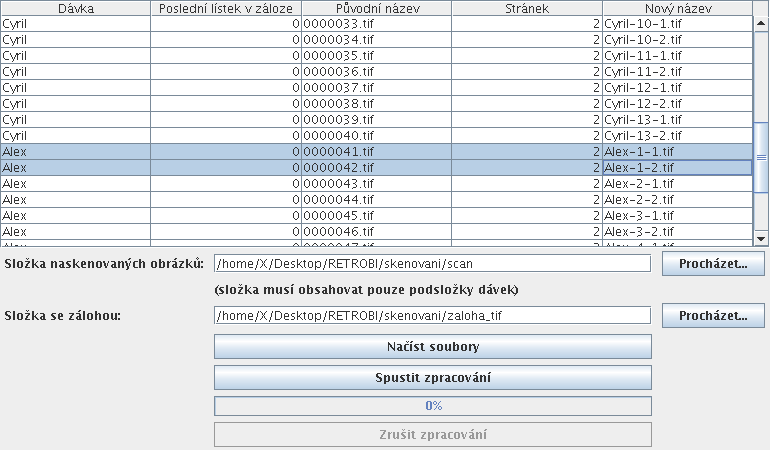
\includegraphics[width=\textwidth]{u1.png}
\caption{Seznam načtených souborů}
\end{figure}

\subsubsection{Import lístků (Udělátko 2 / importer)}

\begin{itemize}
\item{{\bf Vstup:} přejmenované soubory}
\item{{\bf Výstup:} lístky v databázi}
\end{itemize}

Dalším velmi důležitým krokem je import naskenovaných lístků do databáze online katalogu. Naskenované soubory jsou z minulého kroku již přejmenované, prázdné stránky + makulatury jsou smazané a u souborů se volitelně nachází textové soubory s jejich OCR přepisy.

Spusťte druhý nástroj (udělátko 2). Kořenovou složku zálohy vyberete kliknutím na tlačítko \uv{Procházet...}. Poté vyberte složku, do které chcete ukládat výstupní soubory PNG, což jsou zmenšeniny původních obrázků. Do této výstupní složky se každý soubor zkopíruje s celou cestou, relativní k vybrané kořenové složce zálohy.

{\color{OliveGreen} Nástroj kromě TIFFů dokáže načítat i zpracované PNG soubory.}

Poté načtěte soubory tlačítkem \uv{Načíst soubory} a zkontrolujte, zda jsou údaje v tabulce správné a skutečně odpovídají lístkům, které chcete importovat. Indikuje se zde i přítomnost OCR přepisu. Soubory je možné podle tohoto příznaku i řadit (viz checkbox \uv{Řadit dle přítomnosti OCR} dole).

\begin{figure}
\label{fig:u2a}
\centering
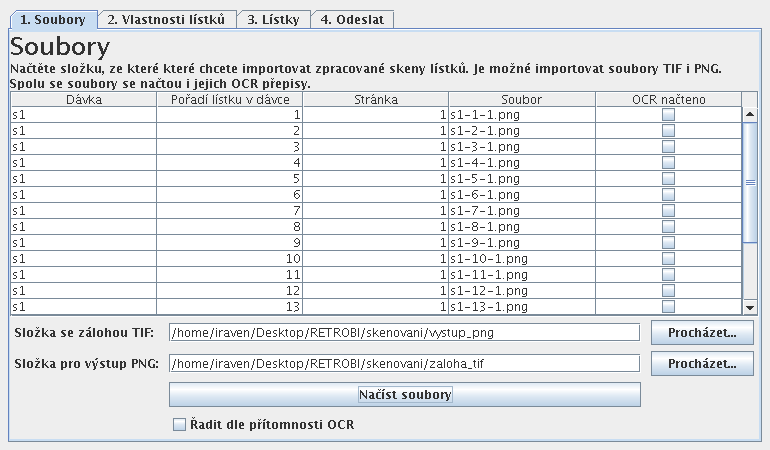
\includegraphics[width=\textwidth]{u2a.png}
\caption{Záložka se soubory}
\end{figure}

Po načtení souborů a kontrole přejděte na další záložku, to jest \uv{Vlastnosti lístků}. Zde vyplňte všechny údaje, které jsou společné všem načteným lístkům. Zpravidla je to \uv{Šuplík}. Dále zadejte své jméno jako hodnotu parametru \uv{Vložil}. To usnadní případné dohledávání. Pomocí prvků v dolní části obrazovky můžete přidávat a odebírat parametry další. Parametry, u kterých je v hodnotě uvedeno \uv{(automaticky)}, doplní nástroj automaticky. Tyto řádky ani nejdou odebrat.

Nakonec nezapomeňte v dolní části vybrat část katalogu.

\begin{figure}
\label{fig:u2b}
\centering
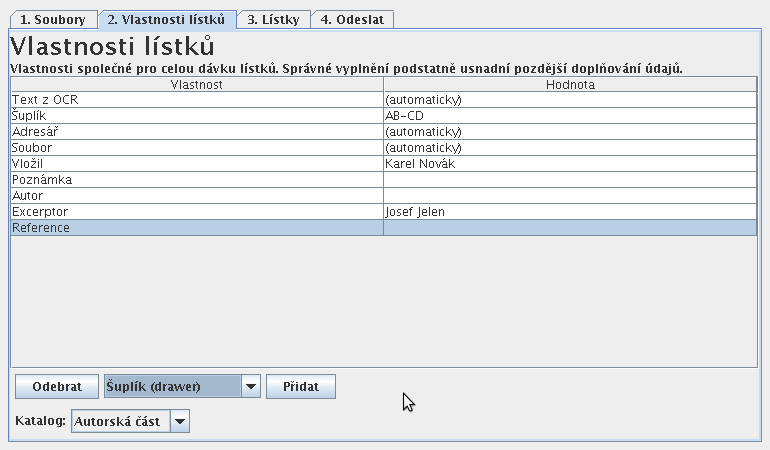
\includegraphics[width=\textwidth]{u2b.png}
\caption{Záložka se společnými vlastnostmi lístků}
\end{figure}

Po vyplnění všech hodnot se můžete přesunout na další záložku \uv{Lístky}. Tato obrazovka slouží především ke kontrole. Jsou zde pod sebou vypsány jednotlivé lístky a konečné hodnoty všech parametrů. Pokud se vám zdá, že je něco špatně, vraťte se na předchozí záložky a hodnoty opravte. Po kontrole pokračujte na záložku poslední.

\begin{figure}
\label{fig:u2c}
\centering
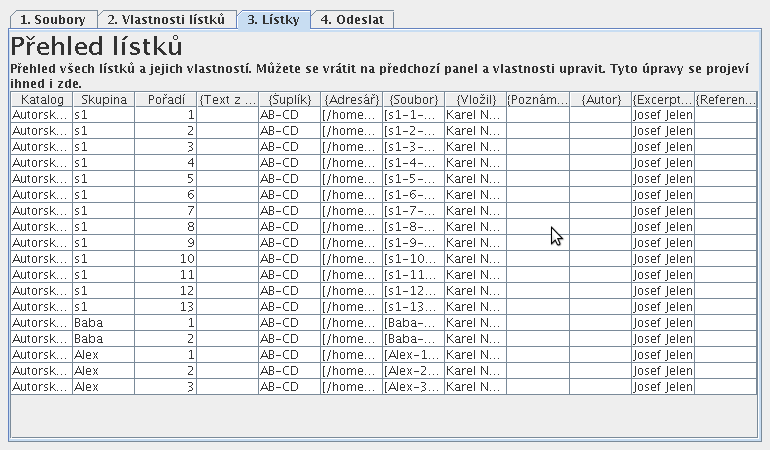
\includegraphics[width=\textwidth]{u2c.png}
\caption{Záložka s přehledem všech lístků}
\end{figure}

Na poslední záložce \uv{Odeslat} je tlačítko \uv{Odeslat na server}, které spustí upload lístků do databáze. Tento proces může chvíli trvat, protože jsou lístky zmenšovány a konvertovány.

Nástroj u každého souboru ověří, zda se již v databázi nenachází. Pokud již soubor v databázi existuje, celý lístek se přeskočí.

{\color{OliveGreen} Dojde-li v tomto procesu k chybě nebo je počítač nečekaně vypnutý, budou se lístky v databázi nacházet jen částečně. Výše popsaný mechanismus detekce duplikátních souborů by měl zamezit opakovanému odeslání stejného lístku.}

\begin{figure}
\label{fig:u2d}
\centering
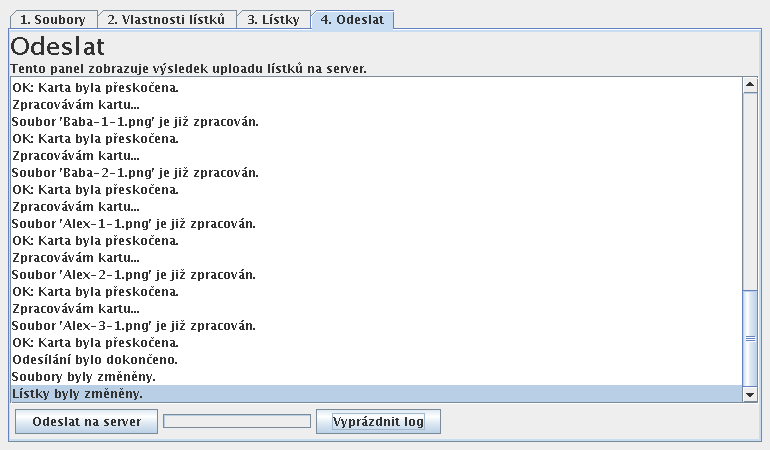
\includegraphics[width=\textwidth]{u2d.png}
\caption{Záložka umožňující upload lístků na server}
\end{figure}

Po dokončení uploadu se zobrazí informační dialog, který obsahuje celkové počty lístků (odesláno, přeskočeno, chyb).

\begin{figure}
\label{fig:u2e}
\centering
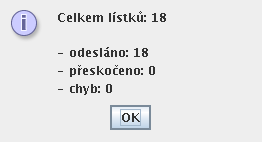
\includegraphics[width=.4\textwidth]{u2e.png}
\caption{Informace o průběhu všech operací}
\end{figure}

Tímto byl import lístků dokončen. Celý proces se opakuje, dokud není vše naskenováno.

\section{Webová aplikace}

Detailní popis webové aplikace se nachází na webu, a to v sekci \uv{Nápověda}. Zde uvedeme pouze stručné shrnutí funkcí a obsažených stránek.

\subsection{Procházení lístků}

Srdcem webové aplikace je procházení lístků, a to v katalogu, ve schránce a ve výsledcích vyhledávání. Procházení katalogu a schránky je podobné -- je k dispozici nějaký pevně daný seznam lístků (v případě katalogu je to zvolená skupina, v případě schránky je to její obsah) a uživatel jím prochází po hierarchicky uspořádaných intervalech. Procházení výsledku vyhledávání se liší tím, že se všechny výsledky nenačítají najednou a neexistuje hierarchie intervalů. Vždy je viditelná pouze nejnižší úroveň, a to jednotlivé lístky.

Tento způsob procházení je podobný přirozenému listování ve fyzické kartotéce. Pokud si otevřeme šuplík s pěti sty lístky a máme za úkol najít lístek č.~134, neprocházíme lístky po jednom. Víme, že je šuplík seřazený a proto se stačí dostat za první stovku, za třetí desítku a nakonec o čtyři lístky dál. 

Procházení po intervalech je podobné. Nejprve zvolíme nejvyšší interval, například tisícovky. Potom volíme stovky, desítky, až nakonec vidíme jednotlivé lístky.

Každý interval lístků je reprezentován zvoleným počtem reprezentantů -- čili lístky, které jsou ze seznamu lístků vybrány po rovnoměrných skocích a zobrazeny uživateli. Dále budeme předpokládat, že požadujeme $S=10$ reprezentantů na interval (tento počet může uživatel ve webové aplikaci měnit na 5, 10, 20, 50, 100). Nižší počet reprezentantů urychluje načítání stránky, ale zároveň zvyšuje počet možných intervalů.

Nyní trochu formálněji. Máme-li tedy k dispozici například $N=1258$ lístků, nejvyšší mocnina $M=S^x$, kde $M<N$ je rovna $M=S^x=10^x=1000 \rightarrow x=3, M=1000$. Nejvyšší intervaly tedy budou mít velikost 1000 a budou to intervaly 1--1000 a 1001--1258. Mezera mezi reprezentanty je 1000, takže mezi každými dvěma z nich se bude nacházet dalších $M-1=1000-1=999$ lístků.

Uživatel si jeden z těchto intervalů vybere, například interval 1--1000. Opět vytvoříme podintervaly s 10 reprezentanty. Vzniknou \uv{nižší} intervaly 1--100, 101--200, a tak dále. Potom je možné mezi intervaly procházet, například \uv{vlevo} od 201--300 je 101--200, \uv{vpravo} je 301--400 a \uv{nahoře} je 1--1000. 

Vlastní způsob reprezentace lístku během procházení si může uživatel měnit. Může si například zobrazit jen vršky lístků, tedy zhruba jejich horní třetinu. Podle ní už se může poměrně dobře v katalogu orientovat a navíc ušetří vertikální prostor na stránce pro další lístky. Zvolit si ale může i kompletní či textové zobrazení.

\subsubsection{Katalog}

Lístky jsou na webu organizovány následovně: katalog obsahuje několik částí. Každá část obsahuje písmena a pod každým písmenem jsou skupiny. Toto členění je vytvořené tak, aby skupiny obsahovaly nejvýše stovky lístků. V celém katalogu se nachází zhruba jeden a půl milionu lístků.

Uživatel po volbě části, písmena a skupiny prochází jednotlivé lístky klasickým intervalovým průchodem, který byl popsán výše.

\subsubsection{Schránka}

Schránka je množina uživatelem vybraných lístků, které \uv{sbírá} při procházení katalogem a výsledků vyhledávání. Tuto množinu může různě organizovat, řadit a měnit. Schránka je uložena v uživatelské relaci (Session), a tak je po jejím zneplatnění ztracena. Uživatel si ji ale může uložit na server anebo na disk. 

Schránku je možné exportovat do dvou formátů: ZIP souboru, který obsahuje jednotlivé obrázky a textové soubory s přepisem (a další), nebo ZIP souboru s velkým RTF dokumentem. 

Schránku lze procházet klasickým intervalovým průchodem, který byl popsán výše.

\subsubsection{Vyhledávání}

Fulltextové vyhledávání začíná v okamžiku, kdy uživatel vyplní vyhledávací formulář a odešle jej. Požadavek je zpracován vyhledávacím servletem CouchDB-Lucene, který provede vlastní vyhledávání. Výsledky jsou poté odeslány zpět webové aplikaci, která je zpracuje a zobrazí, přičemž ve výsledcích zvýrazní \uv{nejlepší} fragmenty, kde došlo k nálezu.

Vyhledávání se zobrazuje jen na úrovni jednotlivých lístků. To znamená, že se vždy zobrazí jen $S$ lístků a není možné přejít o úroveň výš, pouze vlevo a vpravo. 

Je tomu tak z výkonnostních důvodů. Kdyby se celý výsledek nahrál do paměti, mohl by se procházet stejným způsobem jako schránka. Pokud by však bylo výsledků mnoho, například několik set tisíc, omezovaly by množství volné paměti dostupné dalším uživatelům. Také by se značně snížila rychlost vyhledávání, protože by se musely přenést klíče všech nalezených dokumentů. Navíc by se uživatel ve výsledku ani nevyznal. 

Nemožnost procházet výsledky vyhledávání hierarchicky není velká škoda, protože výsledky nejsou seřazeny jako v katalogu, ale zpravidla podle počtu shod s vyhledávacím dotazem.

Výkon vyhledávání dramaticky snižují tzv. {\em divoké karty}, tedy hvězdičky a otazníky. Nejdéle trvá dotaz obsahující výrazy s hvězdičkami z obou stran. Pokud se takových výrazů sejde mnoho, trvá vyhledávání až desítky sekund. Časový limit pro vyhledávání je ale shora omezen (viz konfigurace CouchDB-Lucene a CouchDB výše).

Výsledky vyhledávání je možné přidávat a odebírat ze schránky.

\subsection{Nápověda}

Na webu jsou k dispozici všechny nápovědné texty, které byly vytvořeny na straně ÚČL. Nápovědu lze rozdělit na dvě části: nápověda ke členění katalogu a nápověda k jednotlivým funkcionalitám. Nápovědu lze editovat jako ostatní texty stránek ve správě. Pro jednoduchost zde uvedeme několik nejčastěji používaných XHTML tagů a zápisů. 

\begin{verbatim}
<h1>nadpis</h1> <h2>nadpis</h2> <h3>nadpis</h3>
<p>odstavec</p> <em>kurzíva</em> <strong>tučné</strong>
<a href="url">odkaz</a>
<ul><li>seznam</li></ul> <ol><li>seznam</li></ol>
<table><tr><th>nadpis</th></tr><tr><td>buňka</td></tr></table>
<a href="#sekce">odkaz na sekci</a>
<h3 id="sekce">nadpis sekce</h3>
&quot; = uvozovka
&amp; = amperstand
\end{verbatim}

\subsection{Správa}

Správa je chráněná sekce webu, která je přístupná jen administrátorům a částečně i editorům. Skládá se z několika částí, které umožňují spravovat jednotlivé součásti systému. 

V sekci \uv{Hlášení} se nachází seznam hlášení s filtrem. Hlášení je zde možné potvrzovat a přecházet na jednotlivé lístky. Potvrzená hlášení starší než měsíc je možné stahovat ve formátu CSV a mazat, aby byl v databázi větší pořádek.

V sekci \uv{Hromadná editace} je několik formulářů pro hromadnou změnu lístků ve schránce (přidat hodnotu, odebrat hodnotu, změnit skupinu, odkaz, poznámku, vytvořit nový lístek). Po dokončení hromadné operace jsou ovlivněné lístky rozděleny na dvě skupiny: lístky, u kterých byla změna úspěšně provedena; a lístky, u kterých změna z různých důvodů neproběhla. Změny jsou provedeny pouze v paměti, je tedy možné vzít neuložené změny zpět nebo naopak vybrané změny potvrdit a uložit natrvalo do databáze.

V sekci \uv{Uživatelé} se nachází seznam uživatelů s možností upravit jejich limity a role. Kompletní údaje všech uživatelů (samozřejmě bez hesel) je možné stáhnout ve formátu CSV. Pod tabulkou uživatelů jsou zobrazeny statistiky rolí a institucí, které mají uživatelé nastavené v profilu.

V sekci \uv{Texty} je možné upravovat jednotlivé stránky na webu. Existují dva druhy textů: texty krátké a texty dlouhé. Texty krátké neobsahují žádné formátovací značky, texty dlouhé se zapisují ve formátu XHTML~1.0~Strict. Při editaci doporučujeme \uv{odkoukat}, jak se co zapisuje a hodně napodobovat, není to složité.

V sekci \uv{Analýzy} se nachází nejrůznější přehledy. První část se skládá ze statistik (nejvíce přepisů, počet obrázků), druhá část obsahuje informativní údaje o možných chybách v datech (chybné lístky, skupiny bez prvního lístku, skupiny s nesouvislým číslováním) a přehledy (seznam lístků, u nichž je název skupiny odlišný od názvu skupiny pro řazení, bez citlivosti na velikost písmen).

V sekci \uv{Rejstřík} je roleta s atomickými atributy. Tyto atributy mohou obsahovat hodnoty a je užitečné vědět, jaké různé hodnoty to jsou. K tomu slouží formulář, ve kterém si administrátor vybere atribut a systém mu zobrazí číselník všech různých hodnot tohoto atributu v databázi a počet lístků, které tuto hodnotu obsahují.

V sekci \uv{Nástroje} jsou věci spíše technického charakteru. V první řadě je to seznam CSV logů s možností jejich stažení a možnosti spuštění jednorázových nástrojů pro import dat (tzv. \uv{udělátka}). Následuje informace o posledním a dalším plánovaným spuštění systémové údržby. Pod tím je ještě několik odkazů pro správu systému, které není nutné za normálních okolností aktivovat. Popíšeme si zde, co dělají:

\begin{description}
\item[Znovu načíst a seřadit skupiny:]{Seznam skupin existuje v jedné instanci na celém serveru a všichni návštěvníci jej využívají společně. Protože se struktura katalogu tak často nemění, není nutné ji znovu a znovu při každém požadavku naplňovat. Naplnění je navíc časově náročné. Proto byl vypracován mechanismus, který tuto cache automaticky obnoví jen jednou za den (viz kapitoly o konfiguraci). Kliknutím na tento odkaz ale dojde k okamžitému obnovení této cache, tedy k novému načtení a seřazení všech skupin. Tato operace trvá několik minut.}
\item[Znovu načíst definici atributů a indexů:]{Načte soubor s definicemi položkového rozpisu a znovu vytvoří databázové pohledy a rejstříky. Poté obnovi seznam a vlastnosti vyhledávacích indexů.}
\item[Znovu načíst definici indexů:]{Načte soubor s definicemi dodatečných vlastností vyhledávacích indexů a obnoví jejich seznam.}
\item[Vyčistit indexy:]{Ručně vynutí čištění vyhledávacích indexů, které z nich odstraní nadbytečné informace o již neexistujících dokumentech.}
\item[Optimalizovat indexy:]{Ručně vynutí optimalizaci vyhledávacích indexů. Podrobnosti o této proceduře naleznete v dokumentaci Lucene.}
\item[PING na všechny indexy:]{Odešle krátký testovací vyhledávací dotaz na všechny indexy. Způsobí, že se případné neaktuální indexy začnou na pozadí přepočítávat.}
\item[PING na všechny pohledy:]{Odešle krátký testovací dotaz na všechny databázové pohledy. Způsobí, že se případné neaktuální pohledy začnou ihned přepočítávat. Může trvat až několik hodin (podle toho, kolik pohledů se v průběhu bude aktualizovat).}
\end{description}

Co se seznamu CSV logů týče, bude neustále narůstat. Aby nebyla stránka příliš rychle a zbytečně zahlcena, doporučujeme staré CSV logy pravidelně mazat (přesné umístění složky je zobrazeno nad seznamem logů). Aby je správce systému nemusel mazat ručně, doporučujeme vytvořit automatickou úlohu pro službu CRON. Uvedený skript jednou měsíčně promaže CSV logy starší než 60 dní.

\begin{verbatim}
cd /tmp
echo -n "find CESTA_CSV -mtime +60 -exec rm {} \;" >> rm_old_logs.sh
mv rm_old_logs.sh /etc/cron.monthly/rm_old_logs.sh
\end{verbatim}
